\section{Introduction}
\label{sec:introduction}

\textbf{In this section, the problem will be presented, the motivation behind
the research and the goals of the thesis.}

\textbf{Below are a few examples of how the \LaTeX-document can be used.}

\begin{table}[ht]
    \centering
    \begin{tabular}{@{}rrr@{}}
        \toprule
        Route Size & Time Dijkstra & Search Space \\ \midrule
        59765      & 1330          & 1654488      \\ \hdashline
        124065     & 2405          & 3024948      \\ \hdashline
        111690     & 1523          & 1980856      \\ \hdashline
        52690      & 484           & 645438       \\ \hdashline
        79898      & 2016          & 2512722      \\ \hdashline
        34825      & 532           & 685740       \\ \hdashline
        57301      & 863           & 1100903      \\ \bottomrule
    \end{tabular}
    \caption{I am a sample table}
    \label{tab:sample}
\end{table}

\textbf{Please note: if one would like to use (for whatever reasons) column
separating lines, please avoid using the \textbackslash midrule, \textbackslash
toprule, or \textbackslash bottomrule commands of the booktabs package. A table
realizing vertical lines can be obtained as follows:}

\begin{table}[ht]
    \centering
    \begin{tabular}{|r|r|r|}
        \hline
        Route Size & Time Dijkstra & Search Space \\ \hline
        59765      & 1330          & 1654488      \\ \hdashline
        124065     & 2405          & 3024948      \\ \hline
    \end{tabular}
    \caption{I am a sample table}
    \label{tab:sample2}
\end{table}

\textbf{Various environments can be used to highlight important (theoretical)
parts of the paper. Possible environments are: lemma, definition, corollary,
theorem, observation, remark, example. The numbering is done automatically. The
bracket fills the title (can also be left out).}

\begin{definition}[Sample Definition]
    I am a sample definition.
    \label{def:sample}
\end{definition}

\begin{lemma}[Sample Lemma]
    I am a sample lemma.
    \label{lem:sample}
\end{lemma}

\begin{corollary}[Sample Corollary]
    I am a sample corollary.
    \label{corol:sample}
\end{corollary}

\begin{theorem}[Sample Theorem]
    I am a sample theorem.
    \label{theo:sample}
\end{theorem}

\begin{observation}[Sample Observation]
    I am a sample observation.
    \label{obs:sample}
\end{observation}

\begin{remark}[Sample Remark]
    I am a sample remark.
    \label{rem:sample}
\end{remark}

\begin{example}[Sample Example]
    I am a sample example.
    \label{exa:sample}
\end{example}

\textbf{Algorithms (pseudocode) can look like the following:}

\begin{algorithm}[ht]
    \DontPrintSemicolon
    \KwData{Array $A$}
    \KwResult{Sorted array $A$}
    \BlankLine
    $j:=1$\;
    \While{$j<$length($A$)}{
        $key:=A[j]$\;
        $i:=j-1$\;
        \While{$i >= 0$ and $A[i] > key$}{
            $A[i + 1] := A[i]$\;
            $i--$\;
        }
        $A[i+1]:=key$\;
        $j++$\;
    }
    \caption{INSERTION-SORT($A$)}
    \label{algo:insertion_sort}
\end{algorithm}

\textbf{Images can be included as usual:}

\begin{figure}[ht]
    \centering
    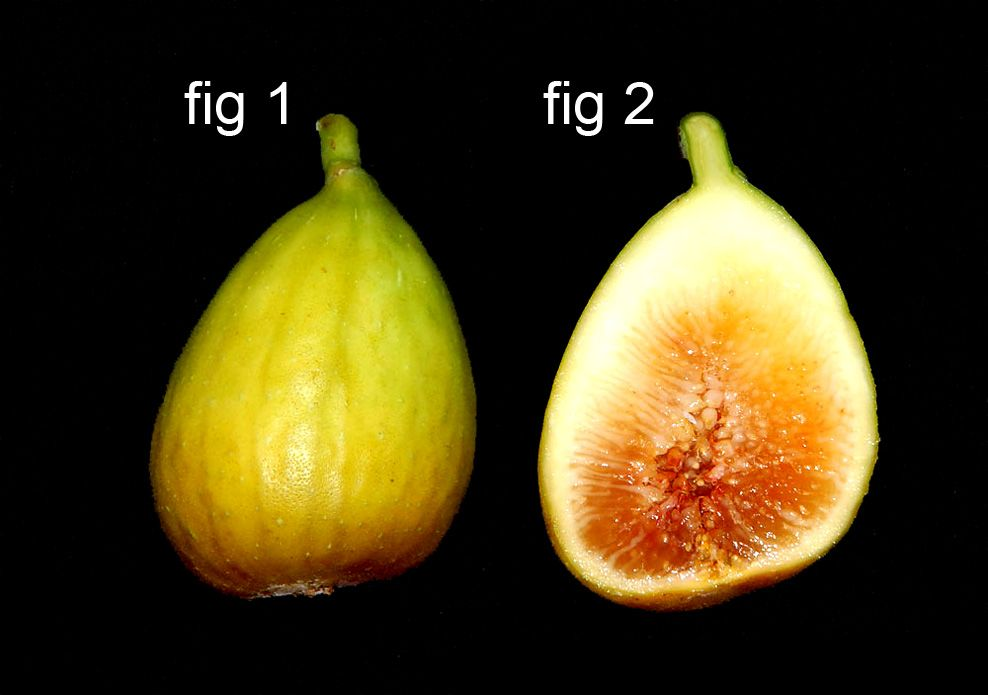
\includegraphics[width=0.5\linewidth]{figures/figs.jpeg}
    \caption{I am a sample figure}
    \label{fig:sample}
\end{figure}

\textbf{If you want to use figures inside definitions, lemmas, etc. Please use:}

\begin{example}
    This is a figure inside an example.

    \begin{statementfigure}
        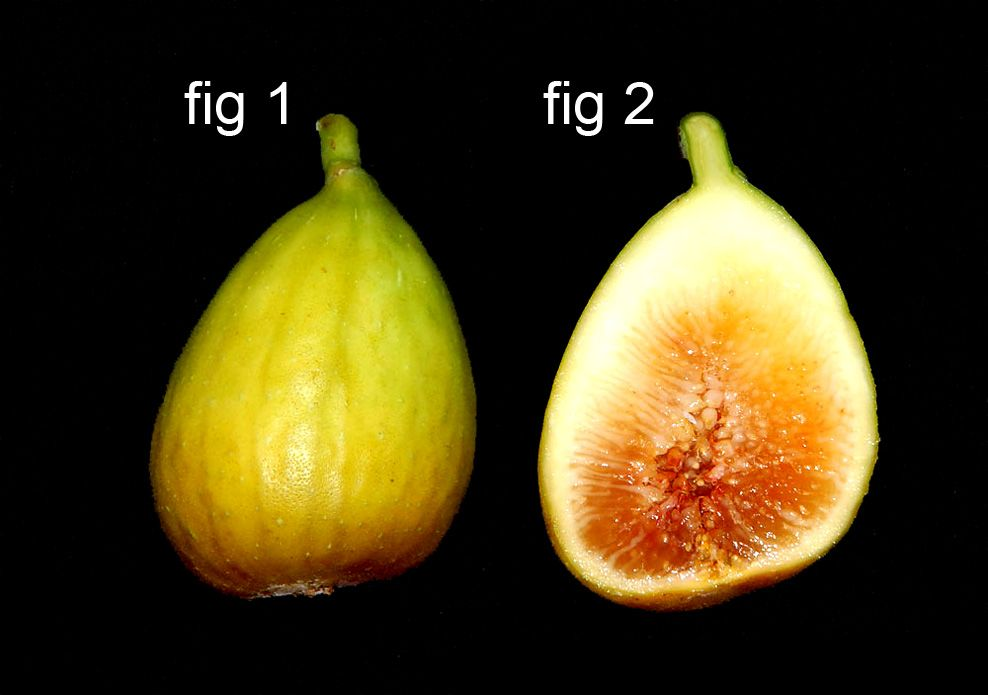
\includegraphics[width=0.25\textwidth]{figures/figs.jpeg}
        \centering
        \caption{Example figure inside statement}
        \label{fig:fig_statement}
    \end{statementfigure}
\end{example}

\textbf{This template is based on the corporate design of the university of
Konstanz, and therefore the official colours of the university can be used.
Below is a list of these colours:}
\begin{center}
    \begin{tabular}{@{}lll@{}}
        \toprule
        Color         & Sample                                      & \LaTeX -Color  \\ \midrule
        Seeblau 20\%  & \textcolor{kn_seeblau20}{\rule{1cm}{0.2cm}} & kn\_seeblau20  \\ \hdashline
        Seeblau 35\%  & \textcolor{kn_seeblau35}{\rule{1cm}{0.2cm}} & kn\_seeblau35  \\ \hdashline
        Seeblau 65\%  & \textcolor{kn_seeblau65}{\rule{1cm}{0.2cm}} & kn\_seeblau65  \\ \hdashline
        Seeblau 100\% & \textcolor{kn_seeblau}{\rule{1cm}{0.2cm}}   & kn\_seeblau    \\ \hdashline
        Seeblau dark  & \textcolor{kn_seeblau_d}{\rule{1cm}{0.2cm}} & kn\_seeblau\_d \\ \hdashline
        Peach 20\%    & \textcolor{kn_peach20}{\rule{1cm}{0.2cm}}   & kn\_peach20    \\ \hdashline
        Peach 35\%    & \textcolor{kn_peach35}{\rule{1cm}{0.2cm}}   & kn\_peach35    \\ \hdashline
        Peach 65\%    & \textcolor{kn_peach65}{\rule{1cm}{0.2cm}}   & kn\_peach65    \\ \hdashline
        Peach 100\%   & \textcolor{kn_peach}{\rule{1cm}{0.2cm}}     & kn\_peach      \\ \hdashline
        Peach dark    & \textcolor{kn_peach_d}{\rule{1cm}{0.2cm}}   & kn\_peach\_d   \\ \hdashline
        Grau 20\%     & \textcolor{kn_grau20}{\rule{1cm}{0.2cm}}    & kn\_grau20     \\ \hdashline
        Grau 35\%     & \textcolor{kn_grau35}{\rule{1cm}{0.2cm}}    & kn\_grau35     \\ \hdashline
        Grau 65\%     & \textcolor{kn_grau65}{\rule{1cm}{0.2cm}}    & kn\_grau65     \\ \hdashline
        Grau 100\%    & \textcolor{kn_grau}{\rule{1cm}{0.2cm}}      & kn\_grau       \\ \hdashline
        Grau dark     & \textcolor{kn_grau_d}{\rule{1cm}{0.2cm}}    & kn\_grau\_d    \\ \hdashline
        Petrol 20\%   & \textcolor{kn_petrol20}{\rule{1cm}{0.2cm}}  & kn\_petrol20   \\ \hdashline
        Petrol 35\%   & \textcolor{kn_petrol35}{\rule{1cm}{0.2cm}}  & kn\_petrol35   \\ \hdashline
        Petrol 65\%   & \textcolor{kn_petrol65}{\rule{1cm}{0.2cm}}  & kn\_petrol65   \\ \hdashline
        Petrol 100\%  & \textcolor{kn_petrol}{\rule{1cm}{0.2cm}}    & kn\_petrol     \\ \hdashline
        Petrol dark   & \textcolor{kn_petrol_d}{\rule{1cm}{0.2cm}}  & kn\_petrol\_d  \\ \bottomrule
    \end{tabular}
    \begin{tabular}{@{}lll@{}}
        \toprule
        Color             & Sample                                          & \LaTeX -Color      \\ \midrule
        Seegruen 20\%     & \textcolor{kn_seegruen20}{\rule{1cm}{0.2cm}}    & kn\_seegruen20     \\ \hdashline
        Seegruen 35\%     & \textcolor{kn_seegruen35}{\rule{1cm}{0.2cm}}    & kn\_seegruen35     \\ \hdashline
        Seegruen 65\%     & \textcolor{kn_seegruen65}{\rule{1cm}{0.2cm}}    & kn\_seegruen65     \\ \hdashline
        Seegruen 100\%    & \textcolor{kn_seegruen}{\rule{1cm}{0.2cm}}      & kn\_seegruen       \\ \hdashline
        Seegruen dark     & \textcolor{kn_seegruen_d}{\rule{1cm}{0.2cm}}    & kn\_seegruen\_d    \\ \hdashline
        Karpfenblau 20\%  & \textcolor{kn_karpfenblau20}{\rule{1cm}{0.2cm}} & kn\_karpfenblau20  \\ \hdashline
        Karpfenblau 35\%  & \textcolor{kn_karpfenblau35}{\rule{1cm}{0.2cm}} & kn\_karpfenblau35  \\ \hdashline
        Karpfenblau 65\%  & \textcolor{kn_karpfenblau65}{\rule{1cm}{0.2cm}} & kn\_karpfenblau65  \\ \hdashline
        Karpfenblau 100\% & \textcolor{kn_karpfenblau}{\rule{1cm}{0.2cm}}   & kn\_karpfenblau    \\ \hdashline
        Karpfenblau dark  & \textcolor{kn_karpfenblau_d}{\rule{1cm}{0.2cm}} & kn\_karpfenblau\_d \\ \hdashline
        Pinky 20\%        & \textcolor{kn_pinky20}{\rule{1cm}{0.2cm}}       & kn\_pinky20        \\ \hdashline
        Pinky 35\%        & \textcolor{kn_pinky35}{\rule{1cm}{0.2cm}}       & kn\_pinky35        \\ \hdashline
        Pinky 65\%        & \textcolor{kn_pinky65}{\rule{1cm}{0.2cm}}       & kn\_pinky65        \\ \hdashline
        Pinky 100\%       & \textcolor{kn_pinky}{\rule{1cm}{0.2cm}}         & kn\_pinky          \\ \hdashline
        Pinky dark        & \textcolor{kn_pinky_d}{\rule{1cm}{0.2cm}}       & kn\_pinky\_d       \\ \hdashline
        Bordeaux 20\%     & \textcolor{kn_bordeaux20}{\rule{1cm}{0.2cm}}    & kn\_bordeaux20     \\ \hdashline
        Bordeaux 35\%     & \textcolor{kn_bordeaux35}{\rule{1cm}{0.2cm}}    & kn\_bordeaux35     \\ \hdashline
        Bordeaux 65\%     & \textcolor{kn_bordeaux65}{\rule{1cm}{0.2cm}}    & kn\_bordeaux65     \\ \hdashline
        Bordeaux 100\%    & \textcolor{kn_bordeaux}{\rule{1cm}{0.2cm}}      & kn\_bordeaux       \\ \hdashline
        Bordeaux dark     & \textcolor{kn_bordeaux_d}{\rule{1cm}{0.2cm}}    & kn\_bordeaux\_d    \\ \bottomrule
    \end{tabular}
\end{center}

\textbf{Use the command \textbackslash knul to \knul{underline} some text.}

\textbf{Use the \enquote{proof} environment to show theoretical proofs:}

\begin{theorem}
    A dog has 9 legs.
\end{theorem}

\begin{proof}
    No dog has 5 legs. A dog has 4 more legs than no dog. From this follows that
    a dog has 9 legs.
\end{proof}


\textbf{Citations and references can be used as follows:}

I am a citation \cite{Beck2020-12-17Puzzl-48882}.

You can cite multiple papers in one command: \cite{bast2013delay,
bast2013result, bast2014frequency, bast2016scalable, bast2020metro,
bast2021metro, Beck2020-12-17Puzzl-48882, eisner2011algorithms,
eisner2011optimal, funke2013polynomial, funke2014k, funke2015automatic}
\cite{storandt2012route, storandt2012quick, storandt2012cruising,
funke2017personal, funke2016deducing, funke2015placement}

\textbf{Tables, figures and algorithms can be referenced with \textbackslash
cref\{$\ldots$\}.}

See \cref{tab:sample}.

See \cref{fig:sample}.

See \cref{algo:insertion_sort}.

\textbf{If you want to reference some theoretical statement, use \textbackslash
cref\{\}}

See some examples at \cref{def:sample} and \cref{lem:sample}.

Blind text:

\lipsum[1-2]


\section{Related Work}
\label{sec:related_work}

\textbf{This section discusses research that is more closely related to the
topic of the paper.}

Blind text:

\lipsum[1-2]


\section{Preliminaries}
\label{sec:preliminaries}

\textbf{This section covers all the requirements that are necessary to
understand the following passages of the paper. Usually, the basic theoretical
foundation of the problem is discussed here.}

Blind text:

\lipsum[1-2]


\section{Algorithm \& Implementation}
\label{sec:algorithm_implementation}

\textbf{This section goes into more detail about the procedures that were used
and how they were implemented. Both the baseline implementation (which has
probably already been covered in the project) and the advanced approach, which
is the main part of the thesis, are explained. Here, you can also already go
into the theoretical runtimes. In addition, it is explained how the theory was
implemented in terms of programming. }

\subsection{Simple Generic Algorithm}
\label{subsec:simple_algo}

Blind text:

\lipsum[1]

\subsection{Refined Generic Algorithm}
\label{subsec:refined_algo}

Blind text:

\lipsum[1]

\subsection{Implementation}
\label{subsec:implementation}

Blind text:

\lipsum[1]


\section{Experimental Evaluation}
\label{sec:evaluation}

\textbf{In this section, the experiments performed (if any) are explained. This
includes how the experiments were set up, how they were performed, and the
conditions under which they were performed. The latter includes both software
environment and hardware environment. It should also be explained on which data
basis these were carried out. In the last subsection of this section, the
results of the experiments are shown.}

\subsection{Experimental Setup}
\label{subsec:exp_setup}

Blind text:

\lipsum[1]

\subsection{Data and Hardware}
\label{subsec:hardware}

\subsubsection{Software and Data}
\label{subsubsec:software}

Blind text:

\lipsum[1]

\subsubsection{Hardware}
\label{subsubsec:hardware}

Blind text:

\lipsum[1]

\subsection{Results}
\label{subsec:results}

Blind text:

\lipsum[1]


\section{Conclusions and Future Work}
\label{sec:discussion_conclusion}

\textbf{This section discusses the conclusions that can be derived from the
experiments presented and from the paper as a whole. Here, the advantages and
disadvantages of the techniques listed are pointed out and an overall conclusion
is drawn. Possible weaknesses of the techniques are also discussed here. Should
the work presented be extended further, this can be described in this section.}

Blind text:

\lipsum[1-2]
